%!TEX root = ../thesis.tex

\section{関連研究}
     Bojarskiら\cite{bojarski}は,カメラ画像と人が操作するステアリングの角度を用いて模倣学習を行うことで,自動車の自動運転に成功している.学習時のシステムを\figref{Fig:bojarski_train}に示す.学習時には,ドライバーが車を運転し,その際に取得したステアリングの角度とカメラ画像を組み合わせてend-to-end学習が行われる.
     これにより,学習後は,\figref{Fig:bojarski_test}に示ようにカメラ画像から直接,ステアリングの角度を出力するシステムになっている.すなわち,カメラ画像のみで自動運転を可能にしている.
     
     \begin{figure}[h]
          \centering
          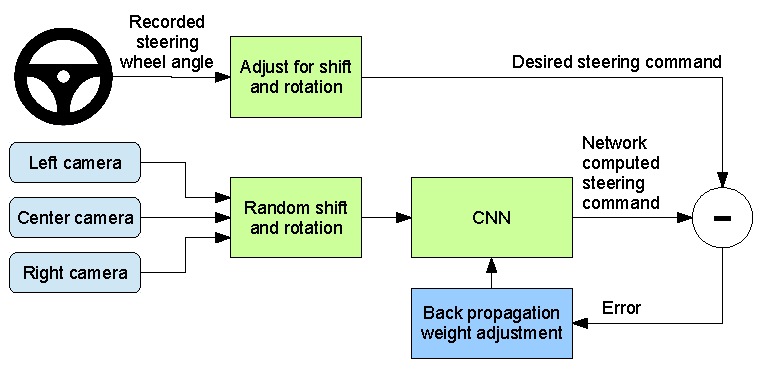
\includegraphics[keepaspectratio, scale=0.16] {images/pdf/bojarski_train}
          \caption[Training the neural network]{Training the neural network (source: \cite{bojarski})}
          \label{Fig:bojarski_train}
     \end{figure}



     \begin{figure}[h]
          \centering
          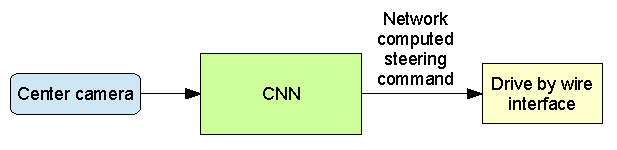
\includegraphics[keepaspectratio, scale=0.20] {images/pdf/bojarski_test}
          \captionsetup{justification=raggedright} % キャプションを左寄せに
          \caption[The trained network is used to generate steering commands from a single front-facing center camera.]{The trained network is used to generate steering commands from a single front-facing center camera. (source: \cite{bojarski})}
          \label{Fig:bojarski_test}
     \end{figure}

\newpage

     \figref{Fig:bojarski_CNN}は,CNNが白線等のない未塗装道路においても,人が操作するステアリングの角度だけを教師信号として用い,有用な道路の特徴を学習したことを示している.なお,道路の輪郭を検出するような学習は明示的に行っていないことが述べられている.

     \begin{figure}[h]
          \centering
          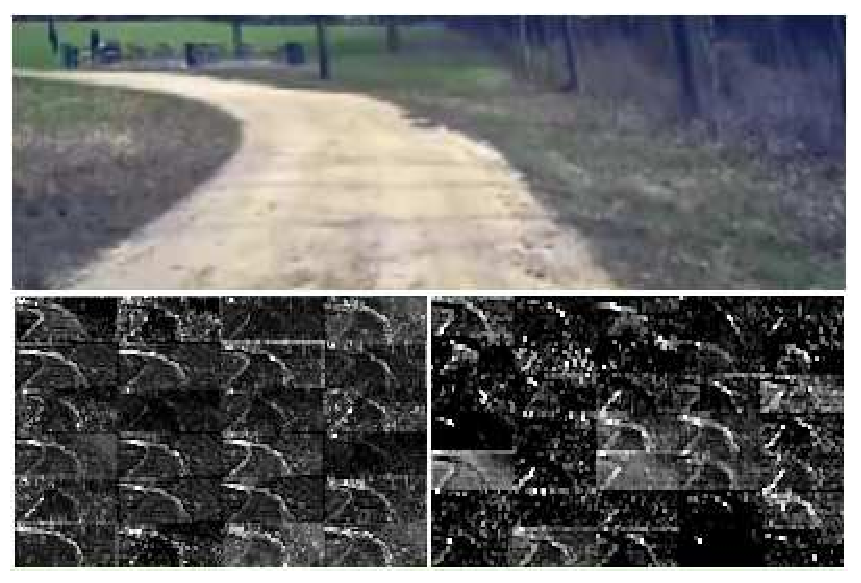
\includegraphics[keepaspectratio, scale=0.35] {images/pdf/bojarski_CNN}
          \captionsetup{justification=raggedright} % キャプションを左寄せに
          \caption[How the CNN ``sees'' an unpaved road. Top: subset of the camera image sent to the CNN. Bottom left: Activation of the first layer feature maps. Bottom right: Activation of the second layer feature maps. This demonstrates that the CNN learned to detect useful road features on its own, i.e., with only the human steering angle as training signal. We never explicitly trained it to detect the outlines of roads.]{How the CNN ``sees'' an unpaved road. Top: subset of the camera image sent to the CNN. Bottom left: Activation of the first layer feature maps. Bottom right: Activation of the second layer feature maps. This demonstrates that the CNN learned to detect useful road features on its own, i.e., with only the human steering angle as training signal. We never explicitly trained it to detect the outlines of roads. (source: \cite{bojarski})}
          \label{Fig:bojarski_CNN}
     \end{figure}

\newpage
